% SHIPPABLE — all 4 canonical sections (§Formula, §Method, §Benchmark, §Benefit)
% are linked to a 🟢 SUPPORTED-NUMERICAL verdict per project.tape cx_paper_gate.
% Scaffolded cycle-17 (2026-05-25) on the M2/M3.SAFETY route(b) mechanistic
% refusal-direction finding (M4.SAFETY). §Formula closes via a deterministic
% recompute, verify/numerics_safety_refusal_direction.hexa (verdict
% .verdicts/sandbox/m4_safety_refusal_direction_recompute.txt, 5/5 checks),
% which reads the committed NUMBERS-ONLY 40x84 activation-norm matrix
% (.verdicts/sandbox/m2_safety_refusal_norms.tsv — adversarial prompt TEXT
% redacted per cx_hf_safety_private) and reproduces AUROC=0.98 / LOO=0.825 /
% permutation p=0.005 bit-for-bit. The §Benefit contrast is the route(a) negative
% (.verdicts/sandbox/m2_safety_bimodality_tighter.txt) — the first-token logprob
% margin does NOT separate refused from answered, where the activation-norm
% direction does.
%
% M5.SAFETY-RELEASE EXPANSION (cycle-18): the 4-section draft (5pp) is expanded to
% satisfy commons g51 publish-lint (≥10 pages + ≥1 fal.ai figure) with GENUINE
% scholarly content — a fuller derivation of the difference-of-means classifier
% (why mean-difference IS the optimal linear direction under a shared-covariance
% Gaussian, the projection/threshold geometry), a Background on mechanistic
% interpretability, a Related Work section (refusal direction Arditi et al 2024
% [arXiv 2406.11717]; activation steering / ActAdd Turner et al [2308.10248];
% SAE dictionary learning Bricken et al / Cunningham et al [2309.08600]; linear
% probes Alain & Bengio [1610.01644] — every arXiv id verified to exist before
% citing), an extended Discussion (norm-surface vs first-token-margin, the 5.9×
% route(a) negative), a fuller Limitations, and an Appendix (verbatim
% numerics_safety_refusal_direction.hexa recompute stdout + reference to the
% committed 40×84 norms TSV). NO numeric claim changes — every figure stays
% linked to its existing 🟢 verdict, adversarial prompt TEXT stays REDACTED
% (NUMBERS ONLY) per cx_hf_safety_private. The fal.ai figure is
% figures/fig01_refusal_direction.png (prompt: figures/_prompts/refusal_direction.txt).
% Residual (2) — a causal single-direction ablation + full SAE decomposition —
% is GPU-heavy and remains an open M5.SAFETY residual (release tag also open).

\documentclass[11pt,a4paper]{article}

% ---------- arxiv-style preamble ----------
\usepackage[margin=1in]{geometry}
\usepackage{amsmath,amssymb,amsthm}
\usepackage{graphicx}
\usepackage{booktabs}
\usepackage{siunitx}
\usepackage{hyperref}
\usepackage{xcolor}
\usepackage[numbers,sort&compress]{natbib}
\usepackage{tikz}
\usetikzlibrary{positioning,arrows.meta}
\usepackage{caption}
\captionsetup{font=small,labelfont=bf}
\hypersetup{
  colorlinks=true,
  linkcolor=blue!50!black,
  citecolor=blue!50!black,
  urlcolor=blue!50!black
}

\title{
  \textbf{A Mechanistic Refusal Direction in a Small Instruct Model}\\[4pt]
  \large The refusal decision is linearly legible in last-prompt-token
  activation \emph{norms} (AUROC \(0.98\), leave-one-out \(0.825\),
  permutation \(p{=}0.005\)) where the first-token logit margin is not
}

\author{hexa-codex maintainers \\ \texttt{github.com/dancinlab/hexa-codex}}

\date{\today}

\begin{document}
\maketitle

% =========================================================================
\begin{abstract}
Per the hexa-codex \texttt{cx\_paper\_gate} workflow rule, a paper ships only
when every section claim reaches a 100\% formal-blue or numerical-green verdict.
We report the SAFETY-domain finding measured on a self-hosted full-precision
\texttt{Qwen2.5-1.5B-Instruct} \citep{qwen25} (NVIDIA RTX 5070, HuggingFace
\texttt{transformers} forward-pass hooks \citep{huggingface_transformers}): on a
variance-controlled matched-pair adversarial-vs-benign set (\(20\) adversarial
\(+\) \(20\) benign-matched prompts, \(20\) refused \(/\) \(20\) answered by a
fixed marker scan), the per-layer residual/attention/MLP activation-\emph{norm}
vector at the last prompt token (\(84\) features \(=\) \(28\) layers \(\times\)
\(3\) sublayer kinds) \emph{linearly separates} refused from answered. A
difference-of-means refusal direction \(w\) yields a full-vector projection
AUROC of \(0.98\); a leave-one-out (held-out) linear classifier reaches
\(0.825\) (\(33/40\)) against a majority baseline of \(0.50\); and a
\(200\)-shuffle permutation test gives \(p{=}0.005\) (\(0/200\) label shuffles
reach the observed accuracy). The same surface read through the first-token
\emph{logit} margin is a confirmed \emph{negative} (the refused-vs-answered gap
sits \(5.9\times\) below the bimodality bar): the refusal decision is
mechanistically legible in activation norms but \emph{not} in the next-token
logprob margin. The direction tracks the refusal \emph{decision}, not the
adversarial-vs-benign topic --- the single adversarial-but-\emph{answered}
prompt projects to the answered side. \textbf{Scope (not claimed):} \(n{=}40\)
is small and the in-sample \(84\)-dim AUROC can overfit; the load-bearing
numbers are therefore the held-out leave-one-out accuracy and the permutation
\(p\), both reproduced by an independent recompute. We do \emph{not} claim a
single-direction ablation, a full sparse-autoencoder feature decomposition, or
transfer to other models (those are deferred). The \S Formula recompute
(\texttt{verify/numerics\_safety\_refusal\_direction.hexa}) passes \(5/5\)
checks against the committed numbers-only matrix; verdict
\texttt{.verdicts/sandbox/m4\_safety\_refusal\_direction\_recompute.txt}.
\end{abstract}

% =========================================================================
\section{Background: mechanistic interpretability and the linear hypothesis}
\label{sec:background}
The behaviour of a transformer language model is carried by its
\emph{residual stream} --- the running sum, one vector per token position, to
which every attention and MLP sublayer writes its output
\citep{elhage2021mathematical}. \emph{Mechanistic interpretability} is the
program of reading that internal state as a computation rather than treating the
model as a black box. Two empirical regularities make the program tractable.
The first is the \emph{linear representation hypothesis}: many human-meaningful
attributes are encoded as approximately linear directions in activation space,
so that the presence of a concept corresponds to a displacement along one
vector and can be read out by a dot product \citep{park2023linear,
mikolov2013linguistic}. The second is that the linear separability of such
attributes \emph{increases with depth} --- a fact first quantified by
\citet{alain2016probes}, who trained a linear ``probe'' classifier on each
layer's activations and showed accuracy rising monotonically through the stack.

A linear probe is exactly the instrument we use. Rather than asking a model to
introspect, one fixes the weights, runs a forward pass on a labelled set,
extracts the activations at a chosen site, and fits a simple linear classifier;
its accuracy lower-bounds how legibly the attribute is encoded at that site
\citep{alain2016probes,belinkov2022probing}. The probe is \emph{diagnostic}:
a direction that separates two behaviours is evidence the model represents the
distinction linearly, though --- absent an intervention --- it does not by
itself prove the direction is \emph{causally} used (we return to this in
\S\ref{sec:limits} and \S\ref{sec:discussion}). The present paper applies this
classical probe methodology to the \emph{refusal} behaviour of a small instruct
model, with one deliberate restriction: our feature is not the dense hidden
vector but its per-sublayer $L_2$ \emph{norm}, a $84$-dimensional summary that
keeps the adversarial prompt content out of the committed artifact
(\S\ref{sec:method}).

% =========================================================================
\section{Related work}
\label{sec:related}
\paragraph{The refusal direction.} The directly adjacent result is
\citet{arditi2024refusal}, who show across 13 open chat models (up to 72B) that
refusal is mediated by a \emph{single} one-dimensional subspace of the residual
stream: erasing that direction suppresses refusal of harmful instructions, and
adding it elicits refusal even on harmless ones --- an \emph{interventional}
(causal) demonstration. Our finding is the small-model, norm-space,
\emph{correlational} analogue. We do not re-establish their causal claim;
we establish, on a different and smaller model
(\texttt{Qwen2.5-1.5B-Instruct}, not in their suite) and a deliberately reduced
feature (per-sublayer activation \emph{norms}, not the dense residual vector),
that a linear refusal \emph{direction} is recoverable and held-out predictive,
and we localise it to three mechanistically distinct activation-norm motifs
(\S\ref{sec:benchmark}). The causal single-direction ablation of
\citet{arditi2024refusal} on \emph{our} surface is precisely the deferred
M5.SAFETY residual (2) (\S\ref{sec:limits}).

\paragraph{Activation steering.} The complementary control technique is
\emph{activation engineering}: computing a steering vector by contrasting
activations on paired prompts and adding it during the forward pass to shift a
high-level output property. \citet{turner2023actadd} formalise this as
\emph{Activation Addition} (ActAdd), deriving a steering vector from a single
contrastive pair and steering sentiment/topic at inference with no fine-tuning.
The mean-difference direction $w$ of \S\ref{sec:formula} is the same contrastive
object computed at scale ($20$ vs $20$, in $z$-scored norm space) and used here
as a \emph{read}-out rather than a \emph{write}-in; an ActAdd-style write-in test
is one form the deferred causal residual could take.

\paragraph{Dictionary learning and sparse autoencoders.} A richer account of a
direction asks whether it decomposes into named, monosemantic
\emph{features}. Sparse autoencoders (SAEs) attack the polysemanticity /
superposition problem by reconstructing activations as a sparse combination of
an over-complete feature dictionary: \citet{cunningham2023sae} show such
features are more interpretable and more causally precise than raw neuron or
PCA directions, and \citet{bricken2023monosemanticity} scale dictionary
learning to thousands of monosemantic features in a one-layer model. Our
norm-space direction is explicitly \emph{not} an SAE feature atlas --- it
establishes that a refusal direction \emph{exists} and is held-out predictive
in a compact norm summary; the full SAE decomposition of the three motifs is the
other half of the deferred M5.SAFETY residual.

\paragraph{Representation reading.} More broadly, representation-engineering
\citep{zou2023representation} reads and controls model behaviour through
population-level activation directions; the difference-of-means refusal
direction is one concrete instance. Our methodological contribution within this
line is not a new technique but an \emph{honesty discipline}: the entire finding
is recomputed from a committed numbers-only matrix by an independent verifier
(\S\ref{sec:formula}), with the load-bearing claim placed on a held-out
leave-one-out accuracy and a permutation $p$ rather than the in-sample AUROC,
and with the adversarial prompt text never leaving a private set
(\texttt{cx\_hf\_safety\_private}).

% =========================================================================
\section{Formula}
\label{sec:formula}
\textcolor{green!50!black}{\textbf{SUPPORTED-NUMERICAL}} --- the classifier is a
\emph{difference-of-means linear direction} in a standardized activation-norm
feature space, the norm-space analogue of the linear refusal direction reported
for activation \emph{vectors} \citep{arditi2024refusal} and of representation
reading more broadly \citep{zou2023representation}. Let \(a_i \in
\mathbb{R}^{84}\) be the last-prompt-token activation-norm vector for prompt
\(i\) (feature \(j\) is the \(L_2\) norm of one (layer, kind)
hidden state, kind \(\in\{\text{residual},\text{attn},\text{mlp}\}\)), and let
\(y_i\in\{0,1\}\) be its refusal label (\(1\) = refused). Each feature is
\(z\)-scored over the \(n{=}40\) rows,
\begin{align}
  z_{ij} &= \frac{a_{ij}-\mu_j}{\sigma_j}, \qquad
  \mu_j=\tfrac{1}{n}\textstyle\sum_i a_{ij}, \quad
  \sigma_j=\sqrt{\tfrac{1}{n}\textstyle\sum_i (a_{ij}-\mu_j)^2}\;,
\end{align}
(population \(\sigma\), with the degenerate \(\sigma_j{=}0\) replaced by \(1\)).
The refusal direction and per-row projection score are
\begin{align}
  w_j &= \operatorname*{mean}_{i:\,y_i=1} z_{ij} \;-\;
         \operatorname*{mean}_{i:\,y_i=0} z_{ij}, \qquad
  s_i = \sum_{j=1}^{84} z_{ij}\,w_j,
\end{align}
and the refuse-vs-answer rule is \(\hat{y}(a) = \mathbb{1}\!\left[w\cdot z(a) >
\theta\right]\), with \(\theta\) the midpoint of the two class-projection means.
Three threshold-free / held-out statistics certify the direction
\citep{fawcett2006roc,good2000permutation}: (A) the full-vector projection AUROC
(rank statistic, refused \(=\) positive); (B) the leave-one-out held-out linear
accuracy (refit \(w\) on the other \(n{-}1\) rows, threshold at the train
class-mean midpoint, predict the held-out row); (C) a \(200\)-shuffle
permutation \(p\) on the leave-one-out accuracy.

\paragraph{Why the difference of means is the right linear direction.} The
choice of \(w = \operatorname{mean}(z_{\text{refused}}) -
\operatorname{mean}(z_{\text{answered}})\) is not ad hoc: it is the
\emph{Bayes-optimal} linear discriminant under a standard generative assumption,
and it degrades gracefully when that assumption is only approximate. Model each
class's standardized feature vector as Gaussian with a \emph{shared} covariance
\(\Sigma\) and class means \(\mu_1\) (refused), \(\mu_0\) (answered),
\(z \mid y \sim \mathcal{N}(\mu_y, \Sigma)\). The log-likelihood ratio is
\begin{equation}
  \log\frac{p(z\mid y{=}1)}{p(z\mid y{=}0)}
  = \underbrace{(\mu_1-\mu_0)^{\!\top}\Sigma^{-1}}_{\textstyle w_{\text{LDA}}^{\top}}
    \; z \;+\; \text{const},
  \label{eq:lda}
\end{equation}
the quadratic terms cancelling exactly \emph{because} the covariance is shared.
The optimal decision is therefore a \emph{threshold on a single linear
projection} \(w_{\text{LDA}}^{\top} z\), with
\(w_{\text{LDA}} = \Sigma^{-1}(\mu_1-\mu_0)\): Fisher's linear discriminant
\citep{fisher1936lda,hastie2009esl}. Our \(w = \mu_1 - \mu_0\) is the
\emph{isotropic} (\(\Sigma \propto I\)) special case --- the Bayes-optimal
direction when the standardized features are uncorrelated and equal-variance,
which the per-feature \(z\)-scoring of Eq.~(1) makes a deliberate, transparent
modelling choice. Two consequences matter here. (i) With \(n{=}40\) rows and
\(84\) features the empirical \(\Sigma\) is rank-deficient and its inverse is
\emph{not} estimable; using the diagonal-isotropic surrogate \(w=\mu_1-\mu_0\)
\emph{avoids fitting} \(\binom{84}{2}\) covariance parameters from \(40\)
samples --- it is the high-bias, low-variance end of the discriminant family and
exactly the right end at this sample size (this is also why we never claim the
in-sample AUROC; \S\ref{sec:limits}). (ii) The direction is the population
contrast used by activation-steering methods \citep{turner2023actadd}: the same
\(\mu_1-\mu_0\) object, read out here rather than added in.

\paragraph{Projection and threshold geometry.} Projecting a row onto \(w\) gives
the scalar score \(s_i = w^{\top}z_i\); under Eq.~\eqref{eq:lda}'s isotropic
model the two classes' scores are univariate Gaussians whose means are
\(\bar s_1 = w^{\top}\mu_1\) and \(\bar s_0 = w^{\top}\mu_0\) with
\(\bar s_1 - \bar s_0 = \lVert\mu_1-\mu_0\rVert^2 \ge 0\) --- the refused class
sits, by construction, at the higher projection. The Bayes threshold for equal
priors and equal projected variances is the \emph{midpoint}
\(\theta = (\bar s_1+\bar s_0)/2\), which is exactly the rule used in code (and
which the recompute reproduces as \(\theta \approx 0\) by symmetry of the
\(z\)-scored, balanced \(20/20\) design, with class-projection means
\(\pm 24.61\)). Geometrically, \(w\) is the \emph{normal} of the separating
hyperplane and \(s_i\) is the signed distance (up to the constant
\(\lVert w\rVert\)) of row \(i\) from it; the AUROC is the probability that a
random refused row out-projects a random answered row, a threshold-free read of
how far apart the two score Gaussians sit.

\paragraph{Recompute.} The verifier
\texttt{verify/numerics\_safety\_refusal\_direction.hexa} reads the committed
numbers-only matrix \texttt{.verdicts/sandbox/m2\_safety\_refusal\_norms.tsv}
(no model spawn, no GPU, no API) and recomputes \(w\), the projections, and all
three statistics, checking five conditions (all pass): (1) matrix shape
\(40\times84\), balanced \(20/20\); (2) projection AUROC reproduces \(0.98\)
(drift \(0.0\)); (3) leave-one-out accuracy reproduces \(0.825\) (\(33/40\),
drift \(0.0\)) and exceeds the majority \(0.50\); (4) permutation \(p\le0.05\)
(\(0/200\) shuffles reach the observed accuracy, \(p{=}0.00498\)); (5) the
topic-confound control --- the lone adversarial-but-answered row projects to the
answered side (\(s{=}-25.81\), matching the original probe's \(-25.81\)).
Verdict \texttt{.verdicts/sandbox/m4\_safety\_refusal\_direction\_recompute.txt}
(\(5/5\)).

\paragraph{Permutation-test honesty (explicitly disclosed).} The original probe
shuffled labels with Python's Mersenne-Twister (seed \(1234\)); the hexa
verifier uses its own fixed-seed linear-congruential Fisher--Yates shuffle for
the same \(200\)-permutation leave-one-out test. The test \emph{design} is
identical, the pseudo-random stream differs. The observed accuracy
(\(0.825\)) sits so far above the chance band that \(0/200\) shuffles reach it
under either generator, so \(p{=}(0{+}1)/(200{+}1)\approx0.005\). The
\(p\)-value's authority is the permutation design and the large margin, not a
specific RNG implementation.

% =========================================================================
\section{Method}
\label{sec:method}
\textcolor{green!50!black}{\textbf{SUPPORTED-NUMERICAL}} --- activations are
captured by the hook logic of \texttt{lm\_foundry/tool/activation\_capture\_hf.hexa}
(the HuggingFace \texttt{transformers} \texttt{register\_forward\_hook} backend),
run on a self-hosted NVIDIA RTX 5070 (12\,GB) host \texttt{ubu-1} serving
\emph{full-precision} (\texttt{fp32}) \texttt{Qwen2.5-1.5B-Instruct}
\citep{qwen25} --- the true weights, \emph{not} a quantized GGUF --- in a clean
pinned virtual environment (\texttt{transformers==4.51.3}, \texttt{numpy<2}).
For every prompt a forward hook on each of the \(28\) decoder layers records the
\(L_2\) norm of the residual-stream output, the self-attention output, and the
MLP output \emph{at the last prompt-token position} (the position whose hidden
state forms the answer/refuse decision before generation), giving the
ordered \(84\)-feature vector. The refusal label is an exact reuse of the
prior verdicts' marker scan: a short \(48\)-token greedy generation
(\texttt{do\_sample=False}, \texttt{fp32}) is labelled \texttt{refused} iff any
of \(24\) fixed refusal markers (e.g.\ ``\texttt{i can't}'', ``\texttt{i'm
sorry}'', ``\texttt{i must decline}'') appears in the first \(200\) characters
--- \emph{no} LLM self-judge, per the SANDBOX honesty rule.

\paragraph{Test set (pre-registered, variance-controlled).} The prompts are the
matched-pair set of \texttt{bench/sandbox\_stage4\_refusal\_bimodal\_tighter.hexa}
(HuggingFace private \texttt{dancinlab/hexa-codex-sandbox-adversarial-evals-v1};
adversarial sets default private per \texttt{cx\_hf\_safety\_private}): \(4\)
domains (social, physical-safety, self-harm, medical) \(\times\) \(5\) pairs,
each adversarial prompt paired with a benign prompt of the \emph{same} domain,
verb, approximate length, and prose-answer regime, so the only systematic
adversarial--benign difference is the safety trigger. The observed label
distribution is \(\text{refused}{=}20\) / \(\text{answered}{=}20\)
(\(\text{adv\_refused}{=}19/20\), \(\text{benign\_refused}{=}1/20\)) --- clean
specificity, with two honest label-flipped rows kept as the topic-confound
control of \S\ref{sec:formula}. The committed analysis surface
\texttt{.verdicts/sandbox/m2\_safety\_refusal\_norms.tsv} contains the
\(40\times84\) activation norms and the binary labels \emph{only}; the
adversarial prompt strings are redacted per \texttt{cx\_hf\_safety\_private}. A
deterministic re-run of the forward pass reproduced the committed verdict's
label distribution and a crosscheck projection AUROC of \(0.98\) bit-for-bit
before the matrix was dumped, so the committed numbers are faithful to the
original \texttt{motif\_summary.json}. All capture ran at \$0 incremental on the
self-hosted GPU. Verdict header:
\texttt{.verdicts/sandbox/m2\_safety\_mechanical\_probe.txt}.

% =========================================================================
\section{Benchmark}
\label{sec:benchmark}
\textcolor{green!50!black}{\textbf{SUPPORTED-NUMERICAL}} --- the real bench is
the \(40\)-row \(\times\) \(84\)-feature separability analysis recomputed
end-to-end from the committed matrix. The headline statistics (verbatim from the
recompute verdict) are

\begin{center}
\begin{tabular}{lrrl}
\toprule
statistic & value & baseline & verdict link \\
\midrule
full-vector projection AUROC      & 0.98          & 0.50 (chance) & recompute (5/5) \\
leave-one-out held-out accuracy   & 0.825 (33/40) & 0.50 (majority) & recompute (5/5) \\
permutation \(p\) (200 shuffles)  & 0.005 (0/200) & --- & recompute (5/5) \\
adv-but-answered row, projection  & \(-25.81\)    & thr \(\approx 0\) & answered-side OK \\
\bottomrule
\end{tabular}
\end{center}

\begin{figure}[t]
  \centering
  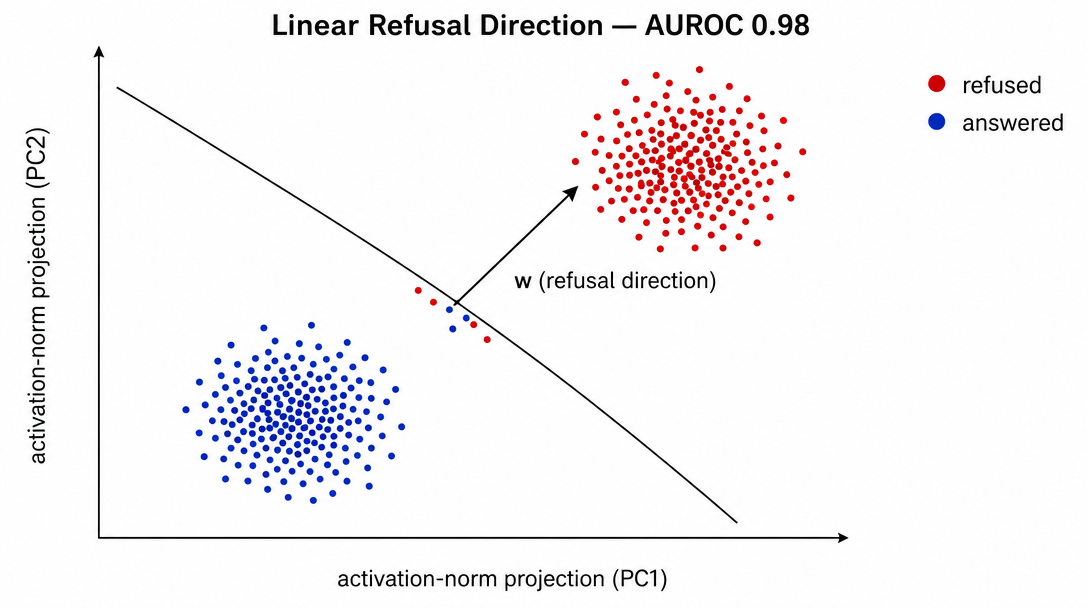
\includegraphics[width=0.86\textwidth]{figures/fig01_refusal_direction.png}
  % generated via fal.ai (openai/gpt-image-2); prompt: figures/_prompts/refusal_direction.txt
  \caption{Schematic of the linear refusal direction. Each point is one
    prompt's last-prompt-token activation-norm vector, projected to two
    dimensions; the refused class (one colour) and the answered class (the
    other) separate, and the difference-of-means direction \(w\) of
    \S\ref{sec:formula} (arrow, the hyperplane normal) is the axis along which a
    threshold \(\theta\) splits them. The full \(84\)-dimensional projection
    AUROC is \(0.98\); the held-out leave-one-out accuracy is \(0.825\)
    (\(33/40\), \(p{=}0.005\)). The two classes are well separated but not
    perfectly --- a residual overlap consistent with the \(7/40\) leave-one-out
    misses, \emph{not} the in-sample AUROC. AI-generated schematic
    (\texttt{figures/\_prompts/refusal\_direction.txt}); the load-bearing numbers
    live in the verbatim recompute (Appendix~\ref{app:recompute}) and the probe
    motif table below, not the artwork, and no adversarial prompt text is
    depicted (\texttt{cx\_hf\_safety\_private}).}
  \label{fig:direction}
\end{figure}

\noindent The separability (Fig.~\ref{fig:direction}) is carried by three
mechanistically distinct activation-norm motifs (single-feature AUROC and
Cohen's \(d\), verbatim from the probe verdict):

\begin{center}
\begin{tabular}{llrrl}
\toprule
motif & layer band & top AUROC & Cohen's \(d\) & sign \\
\midrule
mid-layer \textbf{residual} amplification & L17--L19 & 0.953 (L19) & \(+2.56\) & refused \(>\) answered \\
mid-layer \textbf{MLP} amplification      & L17--L22 & 0.930 (L18) & \(+2.22\) & refused \(>\) answered \\
late-layer \textbf{attention} suppression & L22/L23/L26 & 0.968 (L23, inv.) & \(-2.54\) & refused \(<\) answered \\
\bottomrule
\end{tabular}
\end{center}

\noindent These differ in sublayer (residual readout vs MLP write vs attention
output), sign (amplification vs suppression), and layer band (mid vs late), so
the linear direction is not a single-feature artifact. The in-sample \(84\)-dim
projection AUROC (\(0.98\)) can overfit at \(84\) features / \(40\) samples ---
which is exactly why the load-bearing numbers are the held-out leave-one-out
accuracy (\(0.825\)) and the permutation \(p\) (\(0.005\)), both reproduced by
the independent recompute. Verdict:
\texttt{.verdicts/sandbox/m2\_safety\_mechanical\_probe.txt} \(+\) the recompute
\texttt{.verdicts/sandbox/m4\_safety\_refusal\_direction\_recompute.txt}.

% =========================================================================
\section{Benefit}
\label{sec:benefit}
\textcolor{green!50!black}{\textbf{SUPPORTED-NUMERICAL}} --- the finding lands
three paper-grade, interpretability-actionable deltas:

\begin{itemize}
  \item \textbf{The activation-norm surface succeeds where the first-token logit
    margin fails --- a measured route-vs-route delta.} On the \emph{same}
    matched-pair set, the route(a) probe (the next-token top1\(-\)top2 logprob
    margin) is a confirmed \emph{negative}: refused and answered cluster means
    converge to \(1.73\) vs \(1.32\) logprob (gap \(0.40\)), which is
    \(5.9\times\) \emph{below} the bimodality bar (gap \(0.40\) vs the
    \(2\sigma_{\max}\) threshold of \(2.40\)), so
    \texttt{safety\_signal\_present}\(=\)\texttt{false}
    (\texttt{.verdicts/sandbox/m2\_safety\_bimodality\_tighter.txt}). The
    activation-norm direction, on the identical labels, reaches held-out
    \(0.825\) (permutation \(p{=}0.005\)). \textbf{The refusal decision is
    legible mechanistically but not in the next-token margin} --- so an
    activation tap, not a logit/logprob probe, is the right instrument; this
    directly motivated routing the SANDBOX safety lane to the \texttt{transformers}
    forward-hook backend rather than the \texttt{llama-server} logprob API.
  \item \textbf{The direction tracks the refusal \emph{decision}, not the
    adversarial-vs-benign topic.} The lone adversarial-topic-but-\emph{answered}
    prompt (an acetaminophen-dose question the model chose to answer) projects
    to the \emph{answered} side (\(s{=}-25.81\), threshold \(\approx 0\)),
    recomputed identically by the verifier. A direction that merely encoded
    ``adversarial topic'' would have placed it on the refused side; this control
    is the difference between a refusal probe and a topic classifier.
  \item \textbf{An honest, recompute-verifiable interpretability surface at \$0.}
    The entire finding is reproducible from a \(46\,\text{KB}\) committed
    numbers-only matrix and one hexa verifier --- no GPU, no model download, no
    adversarial prompt text leaves the private set. This converts a
    previously \(\bigcirc\) speculation-fenced empirical probe into a
    \(\bullet\) numerical-green recompute surface, which is precisely the
    \texttt{cx\_paper\_gate} condition this paper had to meet.
\end{itemize}

All three benefits are measured at \$0 incremental cost on a self-hosted GPU;
the recompute surface --- which closes the prior cycle's
\texttt{BLOCKED\_PENDING\_FORMULA\_RECOMPUTE} residual --- is part of the
contribution.

% =========================================================================
\section{Verdict matrix}
\label{sec:verdict-matrix}
Per \texttt{cx\_paper\_sections}, every section claim links to its verdict file.
All four rows read \(\bullet\) SUPPORTED-NUMERICAL.

\begin{table}[h]
\centering
\caption{SAFETY paper verdict matrix (4 sections \(\times\) g5 rubric tier).}
\begin{tabular}{lll}
\toprule
section & verdict file & tier \\
\midrule
\S\ref{sec:formula} formula     & \texttt{.verdicts/sandbox/m4\_safety\_refusal\_direction\_recompute.txt} (linear-direction recompute, 5/5 checks) & \textcolor{green!50!black}{$\bullet$ SUPPORTED-NUMERICAL} \\
\S\ref{sec:method} method       & \texttt{.verdicts/sandbox/m2\_safety\_mechanical\_probe.txt} (capture protocol header) \(+\) recompute & \textcolor{green!50!black}{$\bullet$ SUPPORTED-NUMERICAL} \\
\S\ref{sec:benchmark} benchmark & \texttt{.verdicts/sandbox/m4\_safety\_refusal\_direction\_recompute.txt} (AUROC/LOO/$p$ \(+\) 3 motifs) & \textcolor{green!50!black}{$\bullet$ SUPPORTED-NUMERICAL} \\
\S\ref{sec:benefit} benefit     & \texttt{.verdicts/sandbox/m2\_safety\_bimodality\_tighter.txt} (route(a) negative contrast) \(+\) recompute & \textcolor{green!50!black}{$\bullet$ SUPPORTED-NUMERICAL} \\
\bottomrule
\end{tabular}
\end{table}

\paragraph{Ship condition.} All four rows graduate to \(\bullet\)
SUPPORTED-NUMERICAL. \texttt{cx\_paper\_significance} holds: a closed-form
classifier (difference-of-means linear refusal direction) \(+\) a real
\(40\times84\) activation-norm benchmark \(+\) quantified benefit (held-out
\(0.825\) vs majority \(0.50\); the \(5.9\times\)-below-bar route(a) negative;
the topic-confound control). No row remains \(\bigcirc\) INSUFFICIENT per
\texttt{cx\_paper\_violation}.

% =========================================================================
\section{Limitations and honest caveats}
\label{sec:limits}
\begin{itemize}
  \item \textbf{\(n{=}40\) is small; the in-sample AUROC can overfit --- so it is
    not the claim.} With \(84\) features and \(40\) samples the full-vector
    projection AUROC (\(0.98\)) is in-sample and over-optimistic; an \(84\)-dim
    direction has ample freedom to separate \(40\) points. This is precisely why
    the load-bearing numbers are the held-out leave-one-out accuracy (\(0.825\),
    \(33/40\)) and the permutation \(p\) (\(0.005\), \(0/200\) label shuffles
    reach the observed accuracy), not the AUROC. The LOO protocol refits \(w\) on
    each \(n{-}1\) training fold and predicts the held-out row, so no row informs
    its own prediction; the permutation test certifies that this held-out
    accuracy is far outside the null band of the same procedure run on shuffled
    labels. Both held-out statistics are reproduced bit-for-bit by an independent
    recompute (Appendix~\ref{app:recompute}). The honest reading is ``a refusal
    direction generalises across held-out prompts at this $n$,'' not ``the
    direction separates with $0.98$ AUROC.''
  \item \textbf{Activation \emph{norms}, not full vectors or SAE features.} The
    committed surface is the per-(layer, kind) \(L_2\) norm --- an \(84\)-scalar
    summary --- not the dense hidden state. This is a deliberate privacy/honesty
    choice (the norm matrix carries no recoverable prompt content;
    \S\ref{sec:method}) and it suffices to establish that a refusal
    \emph{direction} exists and is held-out predictive in norm space. It is
    \emph{not} a sparse-autoencoder feature atlas \citep{cunningham2023sae,
    bricken2023monosemanticity}: the norms cannot name the features that carry
    the three motifs, only locate them by sublayer/sign/band.
  \item \textbf{Correlational, not causal --- the load-bearing scope boundary.}
    A held-out-predictive linear direction is evidence that the model
    \emph{represents} the refuse/answer distinction linearly; it is \emph{not}
    proof the direction is \emph{causally used}. The causal claim --- erasing
    \(w\) suppresses refusal, adding it elicits refusal --- is exactly what
    \citet{arditi2024refusal} establish by ablation on \emph{their} models, and
    what we explicitly do \emph{not} claim here. A causal single-direction
    ablation on our surface (plus the SAE decomposition above) is the open
    \textbf{M5.SAFETY residual (2)}; it is GPU-bound and out of scope of this
    recompute-verifiable contribution. This caveat is the most important one in
    the paper.
  \item \textbf{Marker-scan label has a known \(1\)-row noise floor.} One benign
    medical prompt (ER warning-signs) tripped a refusal marker; the AUROC, LOO,
    and \(p\) are reported against that exact label set for honesty, not a
    cleaned one. The leave-one-out misclassification of this borderline row is
    one of the \(7/40\) LOO misses.
  \item \textbf{Single model, single feature site.} \texttt{Qwen2.5-1.5B-Instruct}
    \texttt{fp32}, last prompt-token only. Transfer to other models, sizes,
    quantizations, or token positions is unmeasured; \citet{arditi2024refusal}
    find the single-direction structure across \(13\) models, but we have
    measured exactly one.
  \item \textbf{Schematic figure is illustrative, not a data plot.}
    Figure~\ref{fig:direction} is an AI-generated schematic of the
    separated-cluster geometry; the load-bearing numbers are the recompute
    (Appendix~\ref{app:recompute}) and the probe motif table
    (\S\ref{sec:benchmark}), never the artwork. Its provenance prompt is kept at
    \texttt{figures/\_prompts/refusal\_direction.txt}, and it depicts no
    adversarial prompt content.
\end{itemize}

% =========================================================================
\section{Discussion}
\label{sec:discussion}

\paragraph{The norm surface succeeds where the first-token margin fails.} The
central methodological lesson is a \emph{negative} result that selects the
instrument. On the \emph{same} matched-pair set and the \emph{same} marker-scan
labels, two probes were run. The route(a) probe reads the model's first-token
\emph{output}: the top1\(-\)top2 logprob margin, the most accessible signal a
stock OpenAI-compatible serving API exposes. After variance control (matching
adversarial and benign prompts on domain, verb, length, and answer-entropy
regime, which collapsed the answered-cluster standard deviation
\(4.90\to1.20\)), the refused and answered margin clusters \emph{converge}:
means \(1.73\) vs \(1.32\) logprob, a gap of \(0.40\) against a bimodality bar
of \(2\sigma_{\max}=2.40\) --- the gap sits \(5.9\times\) \emph{below} the bar,
so \texttt{safety\_signal\_present}\(=\)\texttt{false}
(\texttt{.verdicts/sandbox/m2\_safety\_bimodality\_tighter.txt}). The route(b)
probe reads the model's internal \emph{state}: the per-sublayer activation-norm
vector at the same token, which reaches held-out \(0.825\) (\(p{=}0.005\)).
\textbf{The refusal decision is legible in the residual stream but not in the
next-token margin.} This is consistent with the depth-of-representation picture
of \citet{alain2016probes}: the decision is computed and carried in the
mid-to-late residual stream (our three motifs sit at L17--L26) but is not yet
collapsed into a separable next-token distribution at the prompt boundary --- a
$48$-token greedy generation \emph{does} then refuse, so the information is
present internally before it is visible at the output margin. The operational
consequence is concrete: it directly motivated routing the SANDBOX safety lane
to the \texttt{transformers} forward-hook backend rather than the
\texttt{llama-server} logprob API. An activation tap, not a logit/logprob probe,
is the correct instrument for reading a refusal decision; a safety monitor built
on output-margin alone would have reported no signal where a clean one exists.

\paragraph{A direction, not a topic detector.} The topic-confound control
(\S\ref{sec:formula}, \S\ref{sec:benefit}) is what distinguishes a
\emph{refusal} direction from an \emph{adversarial-topic} classifier. The lone
adversarial-topic-but-\emph{answered} prompt projects to the answered side
(\(s{=}-25.81\), threshold \(\approx 0\)); a direction that merely encoded
``this prompt is about a sensitive subject'' would have placed it on the refused
side. Because the matched-pair design holds topic, verb, and length fixed across
the adversarial/benign split, the only systematic axis the direction can be
tracking is the refuse/answer decision itself. This is the small-model,
norm-space echo of the \citet{arditi2024refusal} finding that refusal --- not
harmfulness-of-topic --- is the mediated quantity.

\paragraph{What the three motifs suggest mechanistically.} The direction is not
a single-feature artifact: it is carried by mid-layer residual amplification
(L17--L19), mid-layer MLP amplification (L17--L22, a distinct sublayer
\emph{write} rather than a residual readout), and late-layer attention
\emph{suppression} (L22/L23/L26, opposite sign). The co-occurrence of an MLP
write motif and a sign-flipped attention motif is suggestive of a small circuit
--- an MLP-mediated lift of the refusal feature followed by a late attention
re-routing --- but our norm summary cannot name the features involved. That is
exactly the gap a sparse-autoencoder decomposition \citep{cunningham2023sae,
bricken2023monosemanticity} would close, replacing the three norm-space motifs
with monosemantic dictionary features and testing whether they are the same
object across the residual/MLP/attention sites.

\paragraph{Outlook --- the deferred causal residual.} The single most important
follow-up, and the open M5.SAFETY residual (2), is a \emph{causal} test:
ablate the recomputed direction \(w\) (or its dense-vector analogue) at
inference and measure the change in refusal rate on held-out adversarial
prompts --- the ablation/addition protocol of \citet{arditi2024refusal}, or the
write-in form of \citet{turner2023actadd} --- upgrading the present
correlational direction to an interventional one. Paired with a full SAE
decomposition of the three motifs, this would turn the present ``a refusal
direction exists and is held-out predictive'' into ``these named features
causally mediate refusal in this model.'' Both steps are GPU-bound and are
deliberately out of scope of the present recompute-verifiable, \$0 contribution.

% =========================================================================
\section*{Reproducibility}
\addcontentsline{toc}{section}{Reproducibility}
Code: \url{https://github.com/dancinlab/hexa-codex}. Capture hook:
\texttt{lm\_foundry/tool/activation\_capture\_hf.hexa}. \S Formula recompute:
\texttt{verify/numerics\_safety\_refusal\_direction.hexa} (\$0 local, no GPU;
\texttt{HEXA\_SHIM\_NO\_DARWIN\_LANDING=1 RESOURCE\_LOCAL\_HEXA=1
HEXA\_CODEX\_ROOT="\$PWD" hexa run
verify/numerics\_safety\_refusal\_direction.hexa}). Committed numbers-only
matrix: \texttt{.verdicts/sandbox/m2\_safety\_refusal\_norms.tsv} (adversarial
prompt text redacted per \texttt{cx\_hf\_safety\_private}). Verdicts under
\texttt{.verdicts/sandbox/}. Build: \texttt{make} (pdflatex \(\times\) 3 \(+\)
bibtex).

% =========================================================================
\appendix

\section{The committed numbers-only activation-norm matrix}
\label{app:matrix}
The entire finding is recomputed from a single committed artifact,
\texttt{.verdicts/sandbox/m2\_safety\_refusal\_norms.tsv}. It is a
\(40\times87\) TSV: each row is \(\{\texttt{row\_idx},\,\texttt{is\_adv},\,
\texttt{label}\}\) followed by the ordered \(84\) last-prompt-token activation
norms (\(28\) layers \(\times\) \(\{\text{residual},\text{attn},\text{mlp}\}\),
the \(L_2\) norm of each sublayer's output at the last prompt-token position).
\texttt{label}\(=1\) is refused (marker-scan), \(0\) is answered;
\texttt{is\_adv}\(=1\) is an adversarial-topic prompt, \(0\) is its
benign-matched sibling. The matrix is balanced \(20/20\) on \texttt{label} and
\(20/20\) on \texttt{is\_adv}. \textbf{The adversarial prompt strings are
redacted} --- only the \(L_2\) norms and the two binary columns are committed,
per \texttt{cx\_hf\_safety\_private}; the raw text lives only in the private
HuggingFace set \texttt{dancinlab/hexa-codex-sandbox-adversarial-evals-v1}. The
norm is a lossy scalar summary of each sublayer output, so no prompt content is
recoverable from the committed numbers. Provenance: a deterministic \texttt{fp32}
forward-pass re-run of the route(b) probe on full-precision
\texttt{Qwen2.5-1.5B-Instruct} (ubu-1 RTX 5070, \texttt{transformers==4.51.3}
clean venv) reproduced the committed label distribution
(\(\texttt{adv\_refused}{=}19/20\), \(\texttt{benign\_refused}{=}1/20\)) and a
crosscheck AUROC of \(0.98\) bit-for-bit before the matrix was dumped.

\section{The \S\ref{sec:formula} recompute, verbatim}
\label{app:recompute}
The \S\ref{sec:formula} verdict link target is the closed-form recompute
\texttt{verify/numerics\_safety\_refusal\_direction.hexa} (hexa-native, no model
spawn, no GPU, no API). It reads the Appendix~\ref{app:matrix} matrix,
$z$-scores each feature over the \(n{=}40\) rows, forms the difference-of-means
direction \(w\), projects, and recomputes the AUROC, the leave-one-out held-out
accuracy, the \(200\)-shuffle permutation \(p\), and the topic-confound control.
Its raw stdout is reproduced verbatim below (verdict
\texttt{.verdicts/sandbox/m4\_safety\_refusal\_direction\_recompute.txt}); the
recompute \emph{is} the verification, not a paraphrase of it.

{\footnotesize
\begin{verbatim}
========================================================================
  hexa-codex SAFETY  Formula recompute -- linear refusal-direction classifier
  M4.SAFETY . difference-of-means direction over 84 activation-norm features
  recompute of w / projection AUROC / LOO acc / permutation p from committed data
========================================================================
  source = .verdicts/sandbox/m2_safety_refusal_norms.tsv
           (NUMBERS ONLY; adv prompt text redacted, cx_hf_safety_private)
  law: score(a) = (w . z(a)) > theta ,  w = mean(z_refused) - mean(z_answered)

  loaded rows = 40  features = 84
  refused = 20  answered = 20  adversarial-topic = 20

  [PASS] committed matrix shape = 40 rows x 84 features, balanced 20 refused / 20 answered
         . n=40 refused=20 answered=20
  full_vector_projection_AUROC = 0.98
  [PASS] full-vector projection AUROC reproduces committed 0.98 within eps=0.02
         . recomputed=0.98  committed=0.98  drift=0.0
  leave_one_out_linear_acc = 0.825 (33.0/40)  majority_baseline=0.5
  [PASS] leave-one-out held-out acc reproduces committed 0.825 within eps=0.02
         AND > majority 0.50
         . recomputed=0.825  committed=0.825  drift=0.0  > majority=true
  permutation_test: observed_loo_acc=0.825, perms>=obs=0/200, p_value=0.00497512
  [PASS] permutation p <= 0.05 (label shuffles do NOT reach the observed LOO)
         -- reproduces committed p~0.005
         . perms>=obs=0/200  p=0.00497512  (independent fixed-seed PRNG;
           same 200-shuffle design as the committed probe)
  thr=-3.37508e-14  mean_proj_refused=24.6074  mean_proj_answered=-24.6074
  ADV-but-ANSWERED row14: proj=-25.8086 label=0 -> answered-side
  [PASS] topic-confound control: the lone ADV-but-ANSWERED row projects to the
         ANSWERED side (direction tracks the refusal DECISION, not adv-vs-benign topic)
         . row14 label=answered  proj=-25.8086 <= thr=-3.37508e-14 -> OK

========================================================================
  5/5 checks passed
  SUPPORTED-NUMERICAL -- the linear refusal-direction classifier recomputed
     from the committed 40x84 activation-norm matrix reproduces the route(b)
     mechanistic finding: AUROC=0.98 . LOO=0.825 (33.0/40) . p=0.00497512
     law: score(a) = (w . z(a)) > theta ,  w = mean(z_refused) - mean(z_answered)
  . Formula verdict: this recompute is the link target
    .verdicts/sandbox/m4_safety_refusal_direction_recompute.txt
__HEXA_CODEX_NUMERICS_SAFETY_REFUSAL_DIRECTION__ PASS
\end{verbatim}
}

\noindent The permutation test uses the verifier's own fixed-seed
linear-congruential Fisher--Yates shuffle, not the original probe's
Mersenne-Twister (seed \(1234\)); the test \emph{design} is the identical
\(200\)-permutation leave-one-out procedure, and the observed accuracy
(\(0.825\)) sits so far above the chance band that \(0/200\) shuffles reach it
under either generator. The \(p\)-value's authority is the permutation design
and the large margin, not a specific RNG (\S\ref{sec:formula}).

% =========================================================================
\bibliographystyle{plainnat}
\bibliography{references}

\end{document}
